\chapter{Aufgabe 9}
\section{Aufgabe 9.1}

\paragraph{Aufgabenstellung}
Stellen Sie das Rechtecksignal am Testausgang des Oszi so dar, dass etwa eine Periode den gesamten Bildschirm füllt! (Nicht zwei oder mehr Perioden auf dem Bildschirm.)

\paragraph{Vorüberlegung}
Um ein Signal zu erhalten, kann der eingebaute Signalgenerator verwendet werden. Dieser liefert bereits ein verwendbares Rechtecksignal. Eine Periode besteht aus einen Wellenhoch \& -tief. Damit diese gut sichtbar ist, sollte links und rechts am Bildschirm ein wenig platz sein, ohne dass eine weitere Amplitude zu sehen ist.

\paragraph{Durchführung}
Der Ausgang des Generators wird mit dem BNC-Messeingang auf Kanal 1 verbunden und über die Taste darüber aktiviert. Um das Signal grob auszurichten, wird die Funktion \glqq{}Auto Set\grqq{} verwendet. Anschließend wird die Welle mit dem Horizontalen-Scrollrad gestreckt, sodass nur noch eine Periode sichtbar ist. Eine vertikale Streckung ist hier nun nicht mehr angebracht, da Teile des Signals sonst verschwinden würden.

\begin{figure}
	\centering
	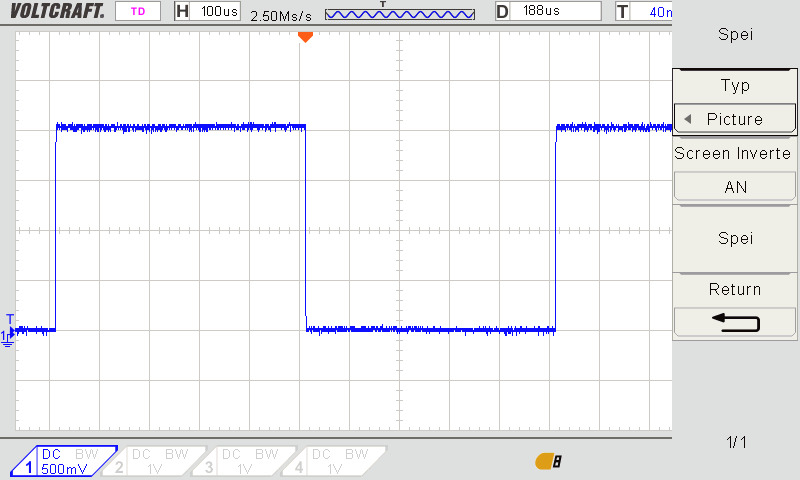
\includegraphics[width=.6\textwidth]{task9-1.jpg}
	\caption{Darstellung einer Periode}
	\label{task9-1}
\end{figure}

\paragraph{Schlussfolgerung}
Die Welle ist nach den Vorgaben eingestellt und wird in Abbildung \vref{task9-1} dargestellt.

\section{Aufgabe 9.2}

\paragraph{Aufgabenstellung}
Zeigen Sie jeweils das Triggern auf steigende und fallende Flanke!

\paragraph{Durchführung}
Über das Triggermenü kann der passende Auslöser eingestellt werden. Um diesen nun Auslösen zu lassen, wird die Erfassung auf \glqq{}Single\grqq{} gestellt und der Kontrollbereich des Triggers, mit dem Einstellrad, hin zur Welle geführt. Berührt der Kontrollbereich das Signal, wird eine Momentaufnahme erstellt.

\begin{figure}
	\begin{minipage}[c]{0.48\linewidth}
		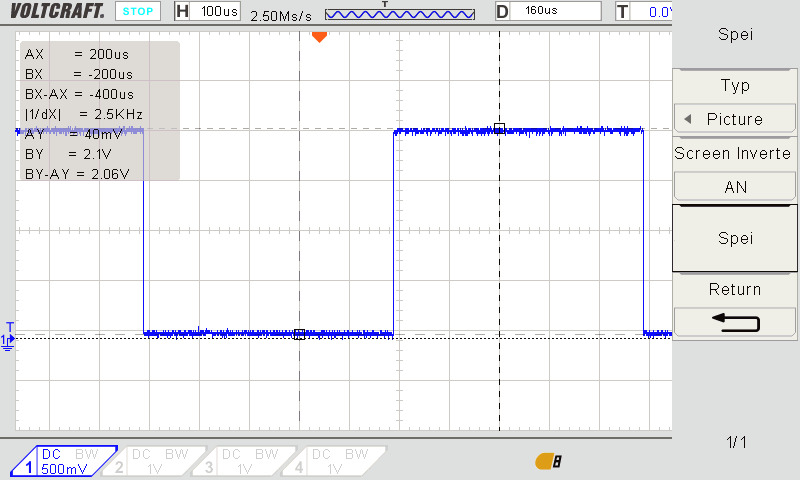
\includegraphics[width=\linewidth]{task9-2-1.jpg}
		\caption{Fallende Flanke}
		\label{task9-2-1}
	\end{minipage}
	\hfill
	\begin{minipage}[c]{0.485\linewidth}
		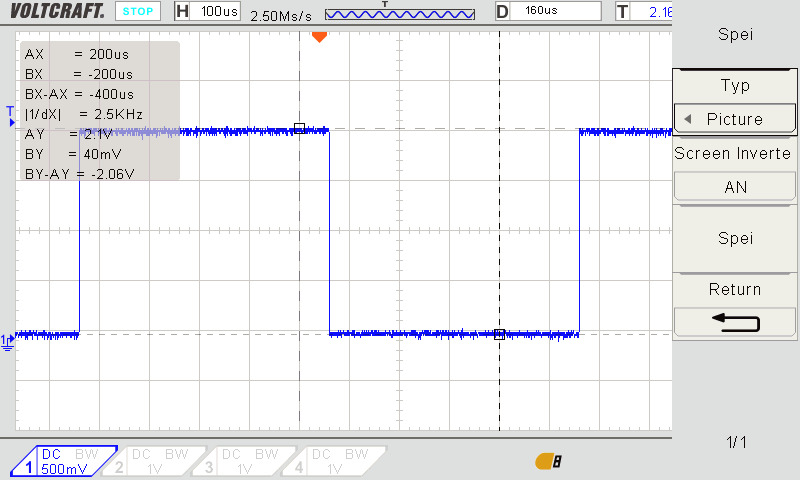
\includegraphics[width=\linewidth]{task9-2-2.jpg}
		\caption{Steigende Flanke}
		\label{task9-2-2}
	\end{minipage}
	\label{task9-2}
\end{figure}

\paragraph{Schlussfolgerung}
Das Auslösen der Ergebnisse war erfolgreich, wie Abbildung \vref{task9-2-1} für die fallende und Abbildung \vref{task9-2-2} für die steigende Flanke zeigen.

\section{Aufgabe 9.3}
\label{task9.3}

\begin{wrapfigure}[9]{r}{.4\textwidth}
	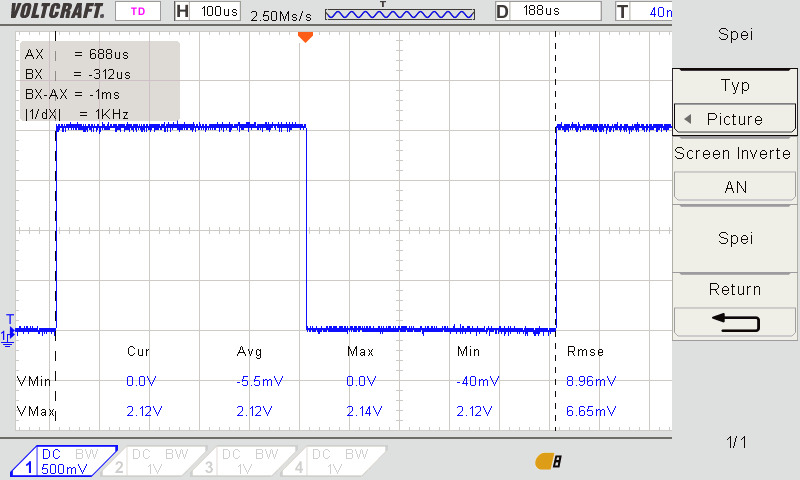
\includegraphics[width=.4\textwidth]{task9-3.jpg}
	\caption{Messung einer Periode}
	\label{task9-3}
\end{wrapfigure}

\paragraph{Aufgabenstellung}
Auf dem Bildschirm des Oszi wird ein Raster erzeugt. Zeigen Sie das Messen der Amplitude und der Periodendauer mit Hilfe des Rasters!

\paragraph{Vorüberlegung}
Die Einheiten für das Raster lassen sich unten Links für jeden Kanal einzeln (Vertikal) und oben links für die gesamte Ansicht (Horizontal) ablesen.

\paragraph{Durchführung}
Für das in Abbildung \vref{task9-3} dargestellte Signal sind es \SI{500}{\milli\volt} auf der Amplitudenachse und \SI{100}{\micro\second} auf der Zeitachse pro Kästchen. Von den Nullstellen bis zum höchsten Ausschlag des Signals befinden sich jeweils zwei Kästchen. Die Amplitude beträgt daher ca. \SI{2}{\volt}. Bei der Periodendauer werden zehn Kästchen gezählt, was \SI{1}{\milli\second} entspricht.

\paragraph{Schlussfolgerung}
Das Ablesen der Werte war erfolgreich, jedoch sind dies nur geschätzte Werte, da exakte Werte nicht mit dem bloßen Auge abgelesen werden können. Dafür müsste man Cursor an der richtigen Stelle einsetzen.

\section{Aufgabe 9.4}

\paragraph{Aufgabenstellung}
Zeigen Sie die Benutzung differentieller und absoluter Cursor auf der Zeit- und der Amplitudenachse! (Im Menüfeld des Oszi befindet sich die Cursor-Taste.)

\begin{wrapfigure}[10]{r}{.4\textwidth}
	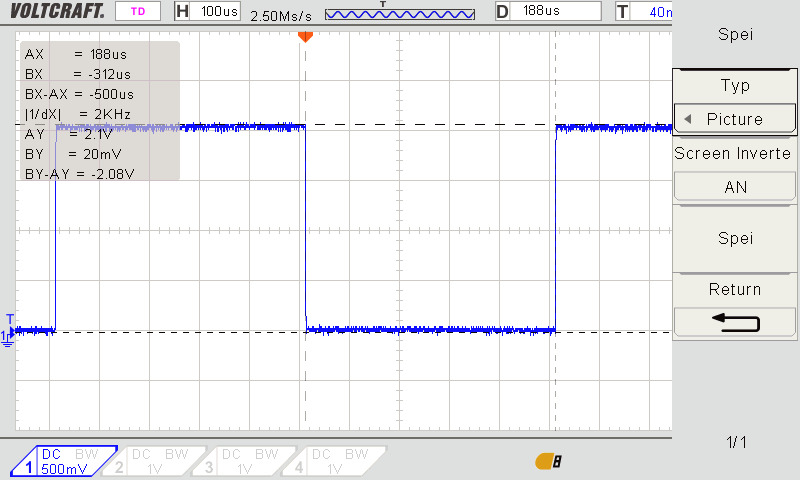
\includegraphics[width=.4\textwidth]{task9-4.jpg}
	\caption{Darstellung einer Periode}
	\label{task9-4}
\end{wrapfigure}

\paragraph{Vorüberlegung}
Pro Achse gibt es jeweils zwei Cursor: A und B. Diese gehören entweder einzeln zu einer Achse, also AX, BX, AY und BY oder bilden ein Paar zu einem differentiellen Cursor, also BX-AX oder BY-AY.

\paragraph{Durchführung}
Im Cursormenü werden nacheinander alle Cursor aktiviert und verwendet. Im das Problem aus \ref{task9.3} zu beheben, werden nun die Cursor an den Amplituden und der Periode ausgerichtet. Durch das Drehen des Menüreglers wird die Position eines Cursors verstellt und dessen Position mit einem Druck fixiert. So könnte man nun die exakten Werte des Signals wie Amplitude oder Periodendauer ermitteln.

\paragraph{Schlussfolgerung}
Die Cursor ließen sich ausrichten und deren aufgezeigte Werte ablesen. Damit lassen sich deutlich präzisere Messwerte ermitteln.